\documentclass[12pt]{article}
\usepackage[margin=1in]{geometry}
\usepackage[all]{xy}

\usepackage{amsmath,amsthm,amssymb,color,latexsym}
\usepackage{geometry}        
\geometry{letterpaper}    
\usepackage{graphicx}
\usepackage[utf8]{vietnam}
\newtheorem{problem}{Problem}
\usepackage{listings}
\usepackage{tcolorbox}
\usepackage{verbatim}
\usepackage{tabularx}
\usepackage{array}
\usepackage{colortbl}
\usepackage{xcolor}
\tcbuselibrary{skins}
\definecolor{Salmon}{RGB}{235,235,235}

\newcolumntype{Y}{>{\raggedleft\arraybackslash}X}

\definecolor{codegreen}{rgb}{0,0.6,0}
\definecolor{codegray}{rgb}{0.5,0.5,0.5}
\definecolor{codepurple}{rgb}{0.58,0,0.82}
\definecolor{backcolour}{rgb}{0.95,0.95,0.92}


\definecolor{blockbackgroundcolor}{RGB}{235,235,235}
\definecolor{blockbordercolor}{RGB}{79,79,79}
\newenvironment{solution}[1][\it{Answer}]{\textbf{#1. } }{}
\lstdefinestyle{mystyle}{
    backgroundcolor=\color{backcolour},   
    commentstyle=\color{codegreen},
    keywordstyle=\color{magenta},
    numberstyle=\tiny\color{codegray},
    stringstyle=\color{codepurple},
    basicstyle=\ttfamily\footnotesize,
    breakatwhitespace=false,         
    breaklines=true,                 
    captionpos=b,                    
    keepspaces=true,                 
    numbers=left,                    
    numbersep=5pt,                  
    showspaces=false,                
    showstringspaces=false,
    showtabs=false,                  
    tabsize=2
}

\tcbset{tab1/.style={fonttitle=\bfseries\large,fontupper=\normalsize\sffamily,
colback=yellow!10!white,colframe=red!75!black,colbacktitle=Salmon!40!white,
coltitle=black,center title,freelance,frame code={
\foreach \n in {north east,north west,south east,south west}
{\path [fill=red!75!black] (interior.\n) circle (3mm); };},}}

\tcbset{tab2/.style={enhanced,fonttitle=\bfseries,fontupper=\normalsize\sffamily,
colback=yellow!10!white,colframe=red!50!black,colbacktitle=Salmon!40!white,
coltitle=black,center title}}

\begin{document}
\graphicspath{ {Figs/} } 

\noindent Trí tuệ nhân tạo - CS106.O21 \hfill DFS/BFS/UCS for Sokoban \\
Nguyễn Hoàng Tân - 21521413

\hrulefill


\begin{problem}
	Sokoban là gì ?
\end{problem}
\begin{solution}
	\begin{itemize}
		\item Sokoban là trò chơi dạng câu đố trong đó người chơi phải
		đẩy một số khối vuông vượt qua chướng ngại vật để đến đích. Trò chơi đã
		được thiết kế vào năm 1981 bởi Hiroyuki Imabayashi và được ra mắt lần
		đầu vào tháng 12 năm 1982.
		\begin{figure}[h]
			\centering
			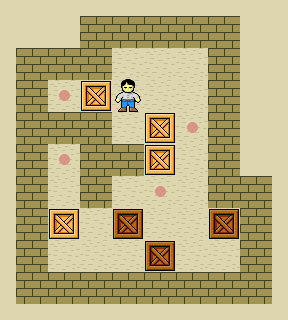
\includegraphics[scale=0.5]{frame_17_delay-0.2s.png}
			% \caption{Sokoban Game from Wikipedia}
		
		\end{figure}
		\item Trong bài tập này, ta sẽ lần lượt sử dụng các thuật toán Uninformed
		Search như DFS, BFS và UCS để giải và so sánh độ hiệu quả của từng thuật toán trên 18 màn chơi.
	\end{itemize}
\end{solution} 

\begin{problem}
	Sokoban đã được mô hình hóa như thế nào ?
\end{problem}
\hspace{-1em}\textbf{1. Biểu diễn bài toán} 
\begin{itemize}
	\lstset{style=mystyle}

	\item Các màn chơi ( level ) sẽ được lưu dưới dạng các txt files, sau đó sẽ được load lên để hiện thị dưới dạng đồ họa 2D bằng cách convert những kí tự trong file text thành một ma trận 2 chiều các số nguyên dương tương ứng.
	
	\begin{tcolorbox}[boxrule=0.5pt, colback=white]
		\begin{lstlisting}[numbers=none, basicstyle=\ttfamily]
		######      ######      ########      #######
		#.  .#      #.  .#      #      #      # .   #
		#    #      #    #      # .XXB&#      # # # #
		# BB #      #B  B#      #      #      #     #
		#&   #      #&   #      #####  #      # B&  #
		######      ######         ####       #######
		\end{lstlisting} 
	\end{tcolorbox}
	
	\lstset{style=mystyle}

	\item Trong đó các kí hiệu tương ứng:
	\begin{itemize}
		\item “\#” là bức tường được biểu diễn là 1.
		\item “B” là các box chưa nằm đúng vị trí được biểu diễn là 3.
		\item “X” là các box đã nằm đúng goal được biểu diễn là 5.
		\item “.” chính là các goal mà ta cần phải đẩy box vào được biểu
		diễn là 4.
		\item “\&” chính là vị trí bắt đầu của người chơi được biểu diễn là 2.
		\item “ “  là các vùng trống được biểu diễn là 0
	\end{itemize}
	\noindent \hspace*{-1em}\textbf{
  Code dùng để convert:}
\begin{tcolorbox}[boxrule=0.5pt, colback=white]
\begin{lstlisting}[language=python, numbers=none, basicstyle=\ttfamily\footnotesize]
	for irow in range(len(layout)):
		for icol in range(len(layout[irow])):
			if layout[irow][icol] == ' ': layout[irow][icol] = 0   
			elif layout[irow][icol] == '#': layout[irow][icol] = 1 
			elif layout[irow][icol] == '&': layout[irow][icol] = 2 
			elif layout[irow][icol] == 'B': layout[irow][icol] = 3 
			elif layout[irow][icol] == '.': layout[irow][icol] = 4 
			elif layout[irow][icol] == 'X': layout[irow][icol] = 5 
	colsNum = len(layout[irow])
\end{lstlisting}
\end{tcolorbox}
\end{itemize}
\hspace{-1em}\textbf{2. Các yếu tố của bài toán tìm kiếm trong Sokoban}
\begin{itemize}
	\lstset{style=mystyle}
	\item Mỗi state mang thông tin liên quan đến vị trí hiện tại của người chơi và boxes
	\item Initial State là vị trí bắt đầu của player và boxes được cung cấp
	\item Trạng thái kết thúc là thời điểm tất cả các goal đều được filled bởi các boxes
	\item Actions: người chơi có thể di chuyển theo 4 hướng (Up, Down, Left, Right) ngoài ra còn có hành động đẩy các boxes ( 1 ô ). 
	\item Từ một state hiện tại, ta có thể sinh ra tối đa 4 state con tùy thuộc vào việc các hành động được tạo ra đó có hợp lệ hay không. Ta có thể xây dựng một kiến trúc cây với các node là những state của bài toán và node gốc là initial state.
	\item Các hành động không hợp lệ có thể bao gồm: di chuyển đụng tường, đầy nhiểu box chồng nhau,... Ta có thể kiểm tra tính hợp lệ của hành động thông qua hàm isLegalAction()
	\newpage
	\noindent \hspace*{-1em}\textbf{
		Ta sinh ra các hành
động bằng hàm LegalActions()}
	\begin{tcolorbox}[boxrule=0.5pt, colback=white]
		\begin{lstlisting}[language=python, numbers=none, basicstyle=\ttfamily\footnotesize]		
def legalActions(posPlayer, posBox):
	"""Return all legal actions for the agent in the current game state"""
	allActions = [[-1,0,'u','U'],[1,0,'d','D'],[0,-1,'l','L'],[0,1,'r','R']]
	xPlayer, yPlayer = posPlayer
	legalActions = []
	for action in allActions:
		x1, y1 = xPlayer + action[0], yPlayer + action[1]
		if (x1, y1) in posBox: # the move was a push
			action.pop(2) # drop the little letter
		else:
			action.pop(3) # drop the upper letter
		if isLegalAction(action, posPlayer, posBox): 
			legalActions.append(action)
		else: 
			continue     

	return tuple(tuple(x) for x in legalActions) # e.g. ((0, -1, 'l'), (0, 1, 'R'))
		\end{lstlisting}
		\end{tcolorbox}
	\item Kết quả trả về là 1 tuple	với 3 thành phần: 2 thành phần đầu là cách di chuyển ứng với tọa độ x và y của player và một
	kí tự để xem bước đi đó có phải là đẩy box hay không ( In hoa biểu thị cho hành động đẩy box)

	\noindent \hspace*{-1em}\textbf{
		Successor function: cập nhật vị trí của player và boxes sau mỗi action}
	\begin{tcolorbox}[boxrule=0.5pt, colback=white]
		\begin{lstlisting}[language=python, numbers=none, basicstyle=\ttfamily\footnotesize]		
def updateState(posPlayer, posBox, action):
	"""Return updated game state after an action is taken"""
	xPlayer, yPlayer = posPlayer # the previous position of player
	newPosPlayer = [xPlayer + action[0], yPlayer + action[1]] # the current position of player
	posBox = [list(x) for x in posBox]
	if action[-1].isupper(): # if pushing, update the position of box
		posBox.remove(newPosPlayer)
		posBox.append([xPlayer + 2 * action[0], yPlayer + 2 * action[1]])
	posBox = tuple(tuple(x) for x in posBox)
	newPosPlayer = tuple(newPosPlayer)
	return newPosPlayer, posBox
		\end{lstlisting}
		\end{tcolorbox}

\end{itemize}

\vspace{1em}
\text{\Huge $\Rightarrow$} Ta có thể sử dụng các thuật toán tìm kiếm trên cây như
DFS, BFS và UCS để tìm \phantom{abcdèfd} đường đi từ state ban đầu tới goal state.
%%%%%%%%%%%%%%%%%%%%%%%%%%%%%%%%%%%%%%%%%%%%%%%%%%%%%%%%
%%%%%Continue with this pattern if there are more%%%%%%%
%%%%%%%%%%%%%%%%%homework problems%%%%%%%%%%%%%%%%%%%%%%
%%%%%%%%%%%%%%%%%%%%%%%%%%%%%%%%%%%%%%%%%%%%%%%%%%%%%%%%

\begin{problem}
	Lập bảng thống kê và so sánh 3 thuật toán DFS, BFS và UCS
\end{problem}
\begin{solution}
	Ta sẽ lần lượt chạy 3 thuật toán trên 18 level cho sẵn và ghi lại kết quả


	\begin{tcolorbox}[tab2,tabularx={X||Y|Y|Y},title=Bảng thống kê thời gian chạy của mỗi thuật toán ứng với từng bản đồ,boxrule=0.5pt]
		\textbf{Level} & \textbf{DFS} & \textbf{BFS} & \textbf{UCS} \\ \hline
		1 & 0.069616 & 0.101242 & 0.052647 \\ \hline
		2 & 0.003891 & 0.009401 & 0.052647 \\ \hline
		3 & 0.253443 & 0.197012 & 0.06424 \\ \hline
		4 & 0.002997 & 0.008998 & 0.00596 \\ \hline
		5 & * & 212.7240 & 56.9723 \\ \hline
		6 & 0.013033 & 0.015529 & 0.003707 \\ \hline
		7 & 0.594837 & 0.964583 & 0.422843 \\ \hline
		8 & 0.084347 & 0.219149 & 0.163834 \\ \hline
		9 & 0.301253 & 0.010904 & 0.010275 \\ \hline
		10 & 0.015936 & 0.018935 & 0.014639 \\ \hline
		11 & 0.020026 & 0.019904 & 0.021127 \\ \hline
		12 & 0.158441 & 0.101224 & 0.072329 \\ \hline
		13 & 0.217540 & 0.166155 & 0.141282 \\ \hline
		14 & 4.335035 & 3.079731 & 2.391904 \\ \hline
		15 & 0.188528 & 0.298266 & 0.224162 \\ \hline
		16 & * & 22.0895 & 13.132285 \\ \hline
		17 & 25.1056 & 24.4073 & 19.932311 \\ \hline
		18 & * & * & * \\ \hline
	\end{tcolorbox}
	\begin{flushleft}
        \textit{Note: “*” là các trường hợp chưa thể đo đạt do các vấn đề về tràn RAM 
		hoặc mất quá lâu để ra kết quả}
        \end{flushleft}
    \label{tab:model_performance}

	\begin{figure}[h]
		\hspace{-3em}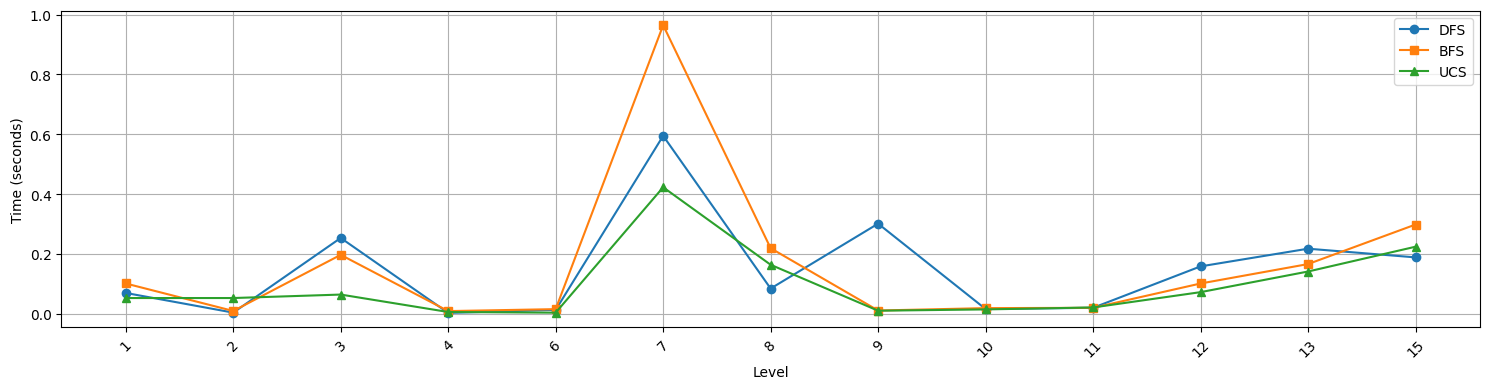
\includegraphics[scale=0.5]{MethodsPerformanceOnEasyLevels.png}
		\caption{Comparison of Algorithm Performance on Easy Levels (Running Time less than 1s)}
	\end{figure}

	\newpage
	Trong những level khó hơn, UCS tỏ ra hiệu quả hơn hẳn 2 thuật toán còn lại. Ở level 5, UCS giải quyết trong vòng 56s trong khi con số này của BFS là 212s và DFS thậm chí gây tràn bộ nhớ. DFS tiếp tục mắc kẹt ở level 16, UCS và BFS lần lượt hoàn thành trong 13s và 22s. Ở level 18 cả 3 thuật toán đều không thể giải quyết.

	\begin{tcolorbox}[tab2,tabularx={X||Y|Y|Y},title=Bảng thống kê số bước di chuyển mỗi thuật toán tìm được,boxrule=0.5pt]
		\textbf{Level} & \textbf{DFS} & \textbf{BFS} & \textbf{UCS} \\ \hline
		1 & 79 & 12 & 12 \\ \hline
		2 & 24 & 9 & 9 \\ \hline
		3 & 403 & 15 & 15 \\ \hline
		4 & 27 & 7 & 7 \\ \hline
		5 & * & 20 & 20 \\ \hline
		6 & 55 & 19 & 5 \\ \hline
		7 & 707 & 21 & 21 \\ \hline
		8 & 323 & 97 & 97 \\ \hline
		9 & 74 & 8 & 8 \\ \hline
		10 & 37 & 33 & 33 \\ \hline
		11 & 36 & 34 & 34 \\ \hline
		12 & 109 & 23 & 23 \\ \hline
		13 & 185 & 31 & 31 \\ \hline
		14 & 865 & 23 & 23 \\ \hline
		15 & 291 & 105 & 105 \\ \hline
		16 & * & 34 & 34 \\ \hline
		17 & 0 & 0 & 0 \\ \hline
		18 & * & * & * \\ \hline
	\end{tcolorbox}
	\begin{flushleft}
        \textit{Note: “*” là các trường hợp chưa thể đo đạt do các vấn đề về tràn RAM 
		hoặc mất quá lâu để ra kết quả. "0" là trường hợp level không có lời giải.}
        \end{flushleft}
    \label{tab:model_numberofmoves}

	\begin{figure}[h]
		\hspace{-3em}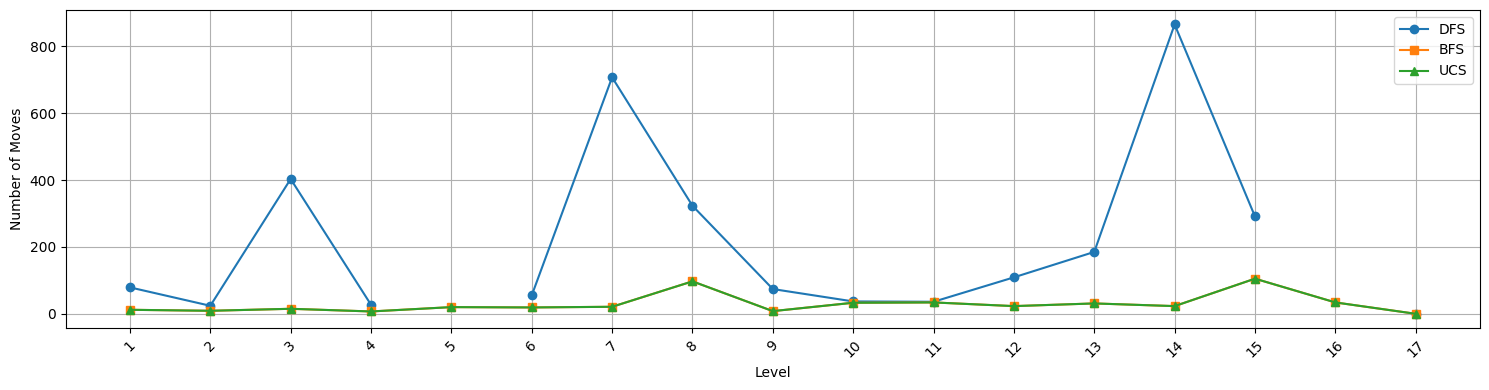
\includegraphics[scale=0.5]{NumberOfMoves.png}
		% \caption{Comparison of Algorithm Performance on Easy Levels (Running Time less than 1s)}
		\begin{flushleft}
			\textit{Ở Level 18, Cả 3 thuật toán đều không tìm ra lời giaỉ (trong thời gian cho phép)}
			\end{flushleft}
	\end{figure}
\end{solution}
\begin{problem}
	Nhận xét về các thuật toán và bản đồ
\end{problem}
\hspace{-1em}\textbf{1. Về các thuật toán} 
\lstset{style=mystyle}

\begin{itemize}
	\item DFS: Kết quả trả về từ thuật toán này không tối ưu và thường rất phức tạp. Đường đi từ initial state đến goal state dài một cách không cần thiết (Đặc biệt ở level 3 khi mà DFS cho ra tận hơn 400 bước đi trong khi đường đi ngắn nhất là 15 bước). Xét đến thời gian chạy, DFS, ở một số level, chạy nhanh hơn 2 thuật toán còn lại (nhưng không đáng kể ), tuy nhiên DFS có thể mắc kẹt vĩnh viễn trong một vòng lặp tại một nhánh khi mà lời giaỉ nằm trong nhánh khác.
	\item BFS: Lời giải của BFS một khi đã tìm được thì sẽ là tối ưu. Tuy nhiên xét về mặt thời gian, do có độ phức tạp là $O(b^d)$ nên BFS thường sẽ mất nhiều thời gian hơn.
	\item UCS: Tìm được lời giải chấp nhận được, trong trường hợp này đều là lời giải tối ưu ( Tuy nhiên nếu chúng ta thay đổi hàm cost thì kết quả có thể sẽ khác). Điểm mạnh của UCS còn nằm ở thời gian thực thi, đa số trường hợp đều vượt trội so với BFS, đặc biệt là những level phức tạp (Việc này có thể bị ảnh hưởng bởi cách ta cài đặt cấu trúc Priority Queue).  
\end{itemize}
\begin{tcolorbox}[boxrule=0.5pt, colback=backcolour]
		Thuật toán hiệu quả nhất theo em là UCS do sở hữu thời gian xử lí nhanh và kết quả tìm được rất tốt
\end{tcolorbox}
\hspace{-1em}\textbf{2. Về các màn chơi đáng chú ý}
\begin{itemize}
	\item Level 5: Thoạt nhìn thì tưởng chừng đây là một level đơn giản, tuy nhiên do kích thước màn chơi quá rộng và trống trải, do đó số lượng legalActions tại mỗi state là quá nhiều. DFS xử lí đã bị mắc kẹt ở một vòng lặp vô tận trong một nhánh quá sâu và khiến bộ nhớ bị tràn. Trong khi đó BFS và UCS chỉ cần mở đến tầng thứ 20 là đã tìm được lời giải tối ưu.
	\item Level 17: Ở màn chơi này, không có cách nào để hoàn thành mục tiêu. Cả 3 thuật toán đều dừng lại sau khoảng hơn 20s.
	\item Level 18: Đây có lẽ là level khó nhất, cấu trúc địa hình rất phức tạp và cả 3 thuật toán đều không thể tìm ra đáp án (trong một khoảng thời gian chấp nhận được).
\end{itemize}

\end{document}
